\documentclass[tikz,border=10pt]{standalone}
% Only base TikZ is needed; no extra libraries.
\begin{document}
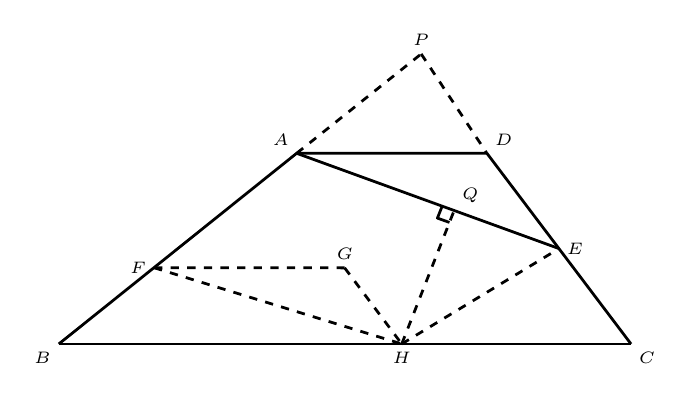
\begin{tikzpicture}[line width=1.0pt, line join=round]
% Coordinates: s = 0.008538 cm/px, origin at image point (543.5, 325)
\coordinate (B) at (-3.633,-1.818);
\coordinate (C) at (3.635,-1.818);
\coordinate (H) at (0.723,-1.817);
\coordinate (A) at (-0.612,0.604);
\coordinate (D) at (1.804,0.605);
\coordinate (E) at (2.720,-0.606);
\coordinate (F) at (-2.423,-0.849);
\coordinate (G) at (-0.002,-0.851);
\coordinate (Q) at (1.388,-0.123);
\coordinate (P) at (0.970,1.866);

% Solid segments
\draw (B) -- (C);
\draw (B) -- (A);
\draw (A) -- (D);
\draw (A) -- (E);
\draw (D) -- (C);

% Dashed segments
\draw[dashed] (A) -- (P);
\draw[dashed] (P) -- (D);
\draw[dashed] (F) -- (G);
\draw[dashed] (G) -- (H);
\draw[dashed] (F) -- (H);
\draw[dashed] (H) -- (E);
\draw[dashed] (H) -- (Q);

% Right-angle mark at Q (one mark only)
\draw (1.236,-0.068) -- (1.176,-0.219) -- (1.329,-0.274);

% Labels
\fontsize{6}{7.2}\selectfont
\node[above left] at (A) {$A$};
\node[above right] at (D) {$D$};
\node[above] at (P) {$P$};
\node[right] at (E) {$E$};
\node[left] at (F) {$F$};
\node[above] at (G) {$G$};
\node[above right] at (Q) {$Q$};
\node[below] at (H) {$H$};
\node[below left] at (B) {$B$};
\node[below right] at (C) {$C$};
\end{tikzpicture}
\end{document}